\section{Results}
\label{sec:Results}

\fix{Nathan and Ron}

\subsection{Memory}
The following memory plots were taken by examining free memory on the nodes
using /proc/meminfo.  Measuring free memory is conservative because it also
accounts for caches and buffers, so although you may run out of free memory in
a system, the execution will not immediately fail due to memory freed from
those other sources.  However, these are an indication of the worst case
possible.  On Cielo there are 16 cores per node and in each case the nodes were
 loaded with 16 MPI ranks executing the statically linked executable.  

In order to understand CTH memory usage results, it is important to note that
CTH preallocates memory based on a value for "max number of blocks" provided
through the input deck.  Because of this, CTH memory usage is highly impacted
by the user specification.  In this case we ran the results with what we
believe are reasonable values for "max number of blocks" given the size of the
problem.  Figure~\ref{fig:MaxBlocks} shows the corresponding max blocks for
each run.

\begin{figure}[htb]
  \centering
  \includegraphics[width=\linewidth]{figures/MemoryUsageInSituPerNode.pdf}
  \caption{Plot of average per node memory usage of the in-situ run on Cielo.}
  \label{fig:MemoryInSituPerNode}
\end{figure}

\begin{figure}[htb]
  \centering
  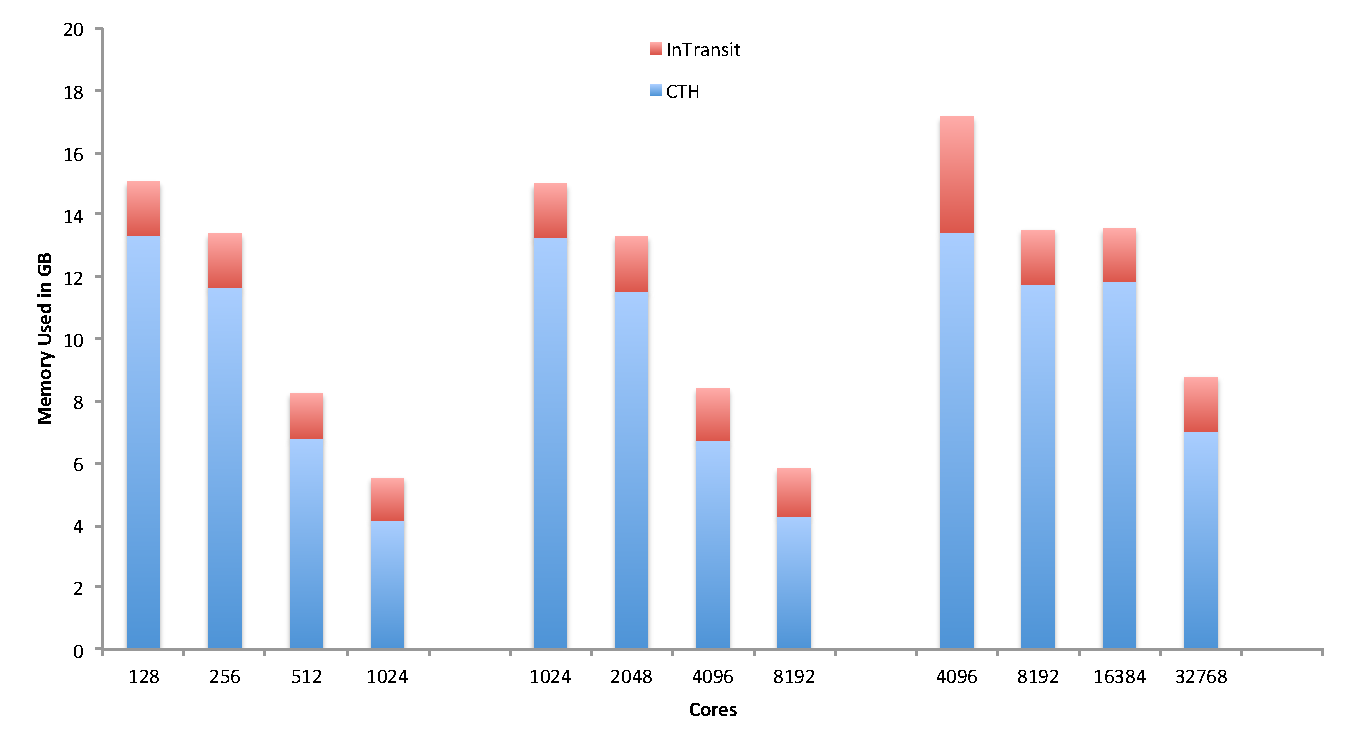
\includegraphics[width=\linewidth]{figures/MemoryUsageInTransitPerNode.pdf}
  \caption{Plot of average per node memory usage of the in-transit run on Cielo.}
  \label{fig:MemoryInTransitPerNode}
\end{figure}

\begin{figure}[htb]
  \centering
  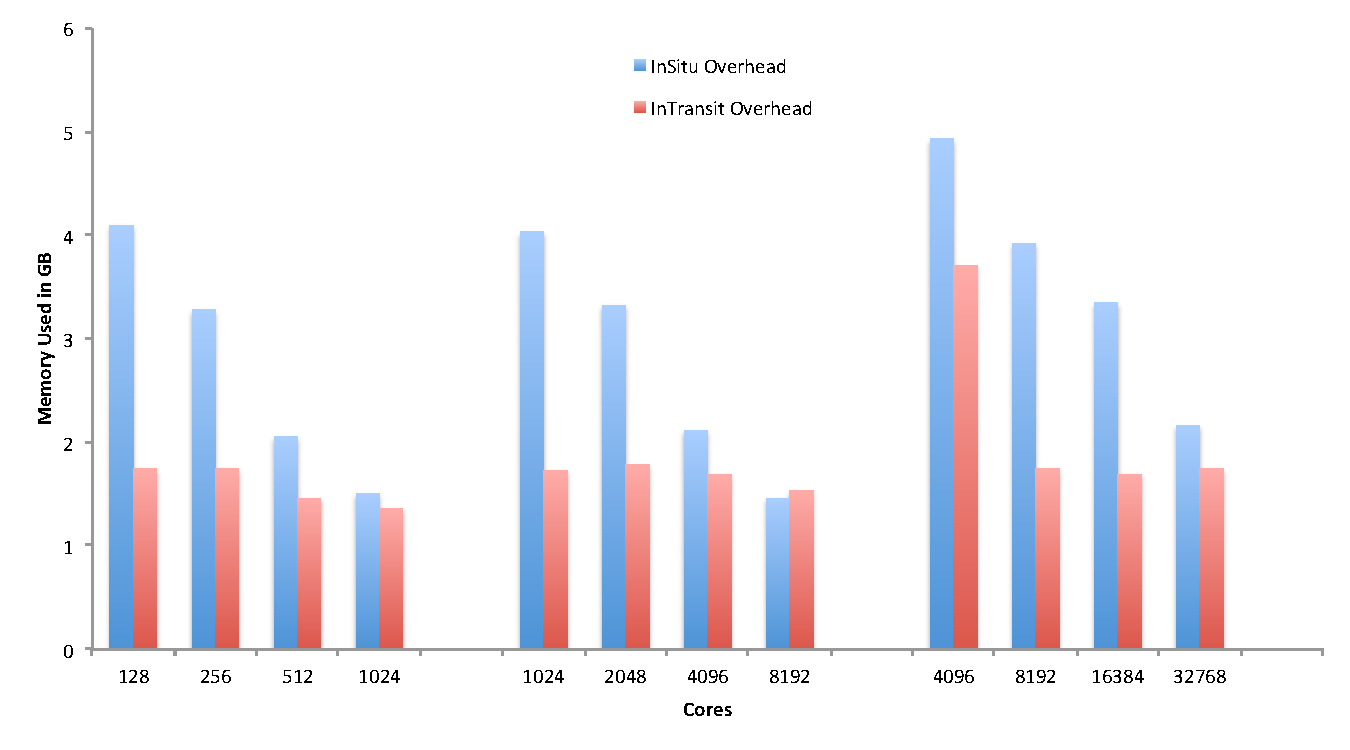
\includegraphics[width=\linewidth]{figures/MemoryUsageCompare.pdf}
  \caption{Plot of the average overhead per node of both InSitu and InTransit}
  \label{fig:MemoryCompare}
\end{figure}

\begin{figure}[htb]
  \centering
  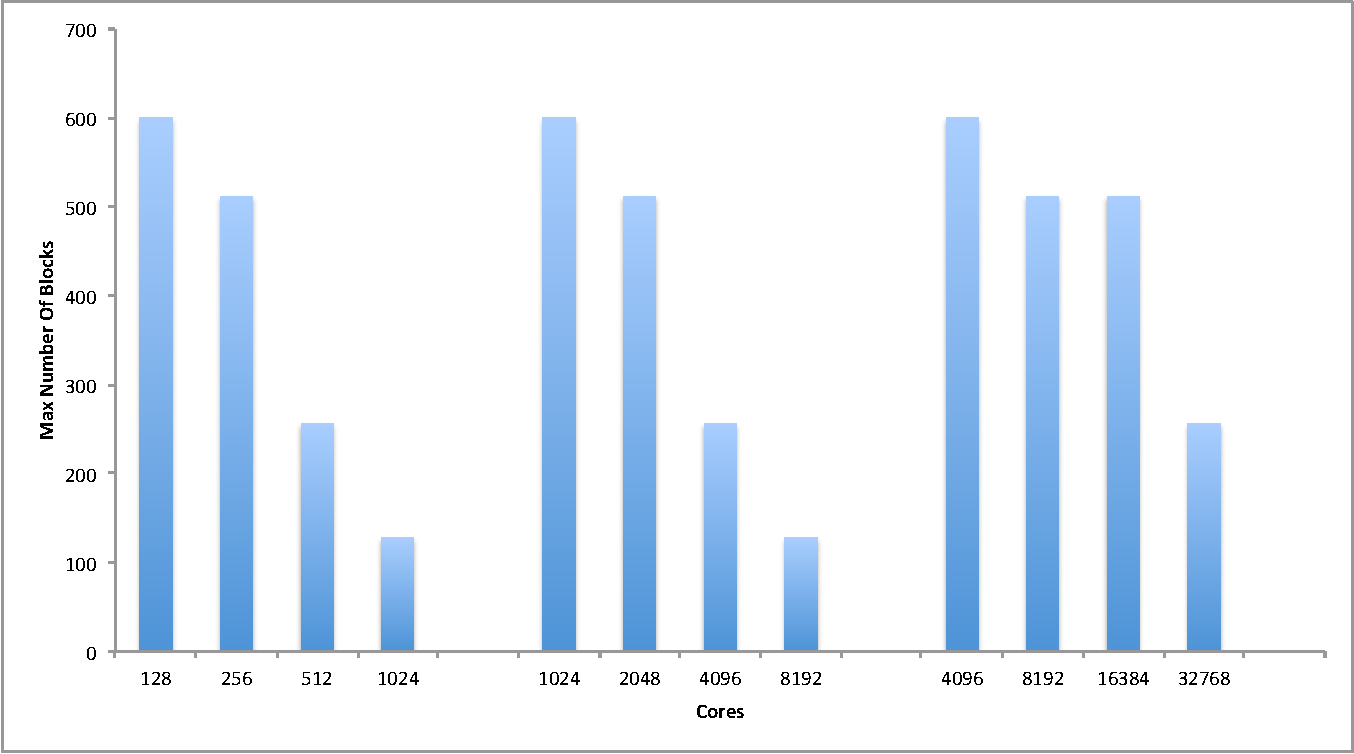
\includegraphics[width=\linewidth]{figures/MaxNumberOfBlocks.pdf}
  \caption{A plot of the "max number of blocks" parameter supplied to CTH for each run.}
  \label{fig:MaxBlocks}
\end{figure}


